\documentclass{article}
\usepackage{amsmath, amssymb, amsthm}
\usepackage{enumitem}
\usepackage{geometry}
\usepackage{tikz}
\usetikzlibrary{arrows.meta, positioning, decorations.pathreplacing, calc}
\usepackage{hyperref}
\usepackage{cleveref}
\usepackage{url}
\geometry{margin=1in}

\newcommand{\doi}[1]{\href{https://doi.org/#1}{\texttt{doi:#1}}}

% ------------------------------------------------------------------
% Theorem environments
% ------------------------------------------------------------------
\newtheorem{theorem}{Theorem}[section]
\newtheorem{lemma}[theorem]{Lemma}
\newtheorem{proposition}[theorem]{Proposition}
\newtheorem{corollary}[theorem]{Corollary}
\theoremstyle{definition}
\newtheorem{definition}[theorem]{Definition}
\newtheorem{example}[theorem]{Example}
\theoremstyle{remark}
\newtheorem{remark}[theorem]{Remark}

% ------------------------------------------------------------------
% Notation
% ------------------------------------------------------------------
\newcommand{\RC}{\mathcal{C}}
\newcommand{\RR}{\mathbb{Z}}
\newcommand{\id}{\mathrm{id}}
\newcommand{\wt}[1]{w(#1)}

\title{A Process-Relational Presentation of Finite Metric Geometry}
\author{Jorge Leonardo Gonz\'alez C\'espedes\\
\small Independent Researcher}
\date{April 2026}

\begin{document}

\maketitle

% ==================================================================
\begin{abstract}
This paper develops a conceptual framework for finite discrete
geometry organized around three commitments: geometric structure
arises from generators and composition laws rather than from a
background space; objects are equivalence classes of finite
processes under a congruence; and metric structure is an external
parameter rather than an intrinsic property of geometric objects.

The mathematical language used throughout is that of quotients
of free categories on weighted directed graphs --- structures
well-established in geometric group theory, the theory of
groupoids, and enriched category theory. The principal
constructions (metric emergence from path optimization, universality
for finite metric spaces, categorical equivalence with Lawvere
metric spaces, Gromov--Hausdorff compatibility) are instances of
known results, recast within this framework and collected in one
place. The relationship to existing work is stated explicitly in
\Cref{sec:related}.

The main contribution of the paper is a \emph{presentation-level
semantic framework}: geometric structure is defined at the level
of generators and congruence laws, prior to quotienting, and
metric properties arise as invariants of congruence classes of
processes. This separates layers --- syntax (generators), laws
(congruence), objects (quotient), and distance (emergent metric)
--- that are usually conflated in classical geometry and in
geometric group theory expositions.

The paper presents a complete isomorphism classification of
single-generator congruences by the pair $(n, k)$
(Proposition~\ref{prop:congclass}). For \emph{non-invertible}
systems this classification is non-trivial: the quotients are
cyclic monoids $M(n,k)$ and the pair $(n,k)$ is a genuine
complete invariant. This is an instance of a classical result in
monoid theory~\cite{cliffordpreston} recast in relational-process
language. For \emph{invertible} systems the constraint $k = 0$
is forced (Corollary~\ref{cor:invertible_classification}), the
pseudo-periodic case does not arise, and the result reduces to
the elementary classification of cyclic groups by order.

The separation of layers makes explicitly askable a question that
classical treatments obscure: what geometric structure does a
specific congruence law produce in the nerve of the free
category, independently of the quotient it defines?
\end{abstract}

% ==================================================================
\section*{Scope and Organization}

A reader familiar with geometric group theory or enriched category
theory will recognize the structures below as weighted directed
graphs, path metrics, and their categorical formulation via
Lawvere's identification of metric spaces with enriched
categories~\cite{lawvere}. The exposition is self-contained: all
definitions are given from scratch, and no prior knowledge of
category theory is assumed. The framework's relationship to
existing work --- including what is reformulated and what is
genuinely new --- is stated in \Cref{sec:related}.

\medskip
\noindent\textbf{Notation.} $V$ denotes a set of states,
$R$ a set of generators, $s, t : R \to V$ source and target maps,
$\RC$ the set of all configurations over $(V, R, s, t)$, and
$\sim$ a congruence on $\RC$. We write $[C]$ for the equivalence
class of a configuration $C$, and $\RC/{\sim}$ for the quotient.
The empty configuration at state $v$ is $\id_v$, written $\id$
when $v$ is clear from context.

% ==================================================================
\section{Relational Systems}
\label{sec:relational}

\begin{definition}[Relational System]
\label{def:relsystem}
A \emph{relational system} is a triple $(V, R, s, t)$ where:
\begin{itemize}
  \item $V$ is a non-empty set of \emph{states},
  \item $R$ is a non-empty set of \emph{generators},
  \item $s, t : R \to V$ are the \emph{source} and \emph{target}
        maps, assigning to each generator a domain and codomain
        state.
\end{itemize}
\end{definition}

\begin{definition}[Compatibility]
\label{def:compat}
Generators $r_1, r_2 \in R$ are \emph{compatible} if
$t(r_1) = s(r_2)$.
\end{definition}

\begin{remark}[Graph structure]
\label{rem:graph}
A relational system $(V, R, s, t)$ is precisely a directed graph
with vertex set $V$ and edge set $R$. Generators are edges;
compatibility is the standard condition for path concatenation;
configurations are directed paths. A weight function
$w : R \to [0,\infty)$ may be added when metric structure is
needed (\Cref{sec:metric}). In \Cref{sec:enriched} this graph
is the generating data for a free enriched category, and the
congruence $\sim$ plays the role of relations in the categorical
sense of a \emph{presentation by generators and relations}.
\end{remark}

% ==================================================================
\section{Configurations as Finite Processes}
\label{sec:configurations}

\begin{definition}[Configuration]
\label{def:configuration}
A \emph{configuration} is a finite sequence of generators
\[
  C = (r_1, r_2, \dots, r_n), \quad r_i \in R,
\]
such that $t(r_i) = s(r_{i+1})$ for each $i = 1, \dots, n-1$
(each consecutive pair is compatible in the sense of
Definition~\ref{def:compat}). The \emph{source} and
\emph{target} of $C$ are $s(C) := s(r_1)$ and $t(C) := t(r_n)$.
The \emph{empty configuration} $\id_v$ at state $v$ (of
length~$0$) satisfies $s(\id_v) = t(\id_v) = v$ and acts as
a two-sided identity. We write $\id$ when the state is clear
from context. The set of all configurations is denoted $\RC$.
\end{definition}

\begin{definition}[Configuration Composition]
\label{def:confcomp}
For $C = (r_1, \dots, r_m)$ and $D = (s_1, \dots, s_n)$ with
$t(C) = s(D)$ (i.e., $t(r_m) = s(s_1)$), their
\emph{composition} is concatenation:
\[
  C \circ D = (r_1, \dots, r_m, s_1, \dots, s_n).
\]
Composition is associative and $\id_v \circ C = C$,
$C \circ \id_v = C$ whenever the sources and targets match.
\end{definition}

\begin{remark}[Configurations are paths]
A configuration is precisely a directed path in the graph
$(V, R, s, t)$ of Definition~\ref{def:relsystem}. Composition
is path concatenation, which is associative by construction.
No further associativity axiom is required.
\end{remark}

% ==================================================================
\section{Congruence and Observational Indistinguishability}
\label{sec:congruence}

\begin{definition}[Congruence]
\label{def:congruence}
An equivalence relation $\sim$ on $\RC$ is a \emph{congruence}
(with respect to composition) if it satisfies:
\begin{enumerate}[label=(\roman*)]
  \item \textbf{Typing preservation.}
        $C_1 \sim C_2$ implies $s(C_1) = s(C_2)$ and
        $t(C_1) = t(C_2)$. Congruent configurations share
        the same source and target state.
  \item \textbf{Composition compatibility.}
        For all $C_1, C_1', C_2, C_2' \in \RC$,
        \[
          C_1 \sim C_1' \;\text{and}\; C_2 \sim C_2'
          \;\Rightarrow\;
          C_1 \circ C_2 \sim C_1' \circ C_2',
        \]
        whenever the compositions are defined.
\end{enumerate}
Typing preservation ensures that the quotient composition
$[C_1] \circ [C_2]$ is well-typed: compatible classes remain
compatible after quotienting.
\end{definition}

\begin{remark}[Practical scope of congruences]
\label{rem:congruence_scope}
The definition above allows arbitrary congruences. In practice,
the paper restricts attention to congruences \emph{generated by
a finite set of relational laws} --- that is, the smallest
congruence containing a given set of pairs $(C_i, C_i')$, closed
under the conditions above. This is the setting of category
presentations. Additional properties --- such as confluence
(the Church--Rosser property) or termination of the associated
rewriting system --- may be imposed when decidability or
algorithmic metric computation is required. Without such
properties, membership in a congruence class may be
undecidable and metric values may be uncomputable. The examples
throughout the paper use finitely generated congruences with
straightforward normal forms.
\end{remark}

\begin{definition}[Observational Indistinguishability]
\label{def:obs-indist}
Given a congruence $\sim$ on $\RC$, configurations $C_1$ and
$C_2$ are \emph{observationally indistinguishable with respect
to $\sim$} if, for every $D \in \RC$:
\[
  C_1 \circ D \sim C_2 \circ D
  \quad\text{(whenever } C_1, C_2 \text{ are left-compatible with } D\text{),}
\]
\[
  D \circ C_1 \sim D \circ C_2
  \quad\text{(whenever } D \text{ is left-compatible with } C_1, C_2\text{).}
\]
\end{definition}

\begin{remark}[Derived property]
\label{rem:no-circularity}
Observational indistinguishability is a consequence of congruence,
not a definition of it. If $C_1 \sim C_2$ and $\sim$ is a
congruence, then for any compatible $D$: $C_1 \circ D \sim C_2 \circ D$
follows immediately from Definition~\ref{def:congruence} applied
with $D \sim D$. The intended workflow is: (1)~fix a relational
system; (2)~specify $\sim$ by listing relational laws;
(3)~verify Definition~\ref{def:congruence}; (4)~conclude that
equivalent configurations are observationally indistinguishable.
\end{remark}

\begin{definition}[Relational Inverse]
\label{def:inverse}
Given a relational system $(V, R, s, t)$ with congruence $\sim$,
a generator $r \in R$ has an \emph{inverse} $r^{-1} \in R$ if:
\[
  (r, r^{-1}) \sim \id_{t(r)}
  \quad\text{and}\quad
  (r^{-1}, r) \sim \id_{s(r)}.
\]
A relational system is \emph{invertible} (with respect to $\sim$)
if every generator has an inverse. Note that $r^{-1}$ must satisfy
$s(r^{-1}) = t(r)$ and $t(r^{-1}) = s(r)$ for the configurations
$(r, r^{-1})$ and $(r^{-1}, r)$ to be well-formed.
\end{definition}

% ==================================================================
\section{Objects and the Quotient Construction}
\label{sec:quotient}

\begin{definition}[Object]
\label{def:object}
An \emph{object} is an equivalence class $[C]$ of a configuration
$C$ under a congruence $\sim$:
\[
  [C] = \{ C' \in \RC \mid C' \sim C \}.
\]
The set of all objects is the quotient $\RC/{\sim}$.
\end{definition}

\begin{remark}[Terminology and categorical context]
\label{rem:objmorph}
In the categorical language of \Cref{sec:enriched}, the equivalence
classes $[C]$ are \emph{morphisms} in the quotient category, while
the states $V$ of the relational system serve as categorical
\emph{objects}. The term ``object'' is used here in the geometric
sense---an equivalence class of processes that no relational test
can distinguish---not in the categorical sense. The two usages are
reconciled in \Cref{sec:enriched}.
\end{remark}

\begin{theorem}[Quotient Construction]
\label{thm:quotient}
Let $(V, R, s, t)$ be a relational system with configuration
set $\RC$, and let $\sim$ be a congruence on $\RC$. Then:
\begin{enumerate}[label=(\roman*)]
  \item\label{qt:wdef} The quotient $\RC/{\sim}$ is well-defined
        as a set of equivalence classes.
  \item\label{qt:comp} Composition descends to a well-defined
        partial operation on $\RC/{\sim}$: whenever $t(C_1) = s(C_2)$,
        \[
          [C_1] \circ [C_2] \;:=\; [C_1 \circ C_2].
        \]
  \item\label{qt:assoc} The induced composition is associative.
  \item\label{qt:id} For each state $v \in V$, the class $[\id_v]$
        acts as a two-sided identity for all classes $[C]$ with
        $s(C) = v$ or $t(C) = v$.
\end{enumerate}
\end{theorem}

\begin{proof}
\textbf{\ref{qt:wdef}.} $\sim$ partitions $\RC$ into disjoint
non-empty equivalence classes.

\textbf{\ref{qt:comp}.} Suppose $[C_1] = [C_1']$ and
$[C_2] = [C_2']$, i.e., $C_1 \sim C_1'$ and $C_2 \sim C_2'$.
Since $\sim$ is a congruence, $C_1 \circ C_2 \sim C_1' \circ C_2'$,
so $[C_1 \circ C_2] = [C_1' \circ C_2']$. The operation is
independent of representatives. Compatibility of $[C_1]$ and
$[C_2]$ is inherited from the compatibility of their
representatives.

\textbf{\ref{qt:assoc}.} For $C_1, C_2, C_3 \in \RC$, associativity
at the configuration level gives
$(C_1 \circ C_2) \circ C_3 = C_1 \circ (C_2 \circ C_3)$.
By part~\ref{qt:comp}:
\[
  ([C_1] \circ [C_2]) \circ [C_3]
  = [(C_1 \circ C_2) \circ C_3]
  = [C_1 \circ (C_2 \circ C_3)]
  = [C_1] \circ ([C_2] \circ [C_3]).
\]

\textbf{\ref{qt:id}.} For any $C$ starting at $v$,
$\id_v \circ C = C$, hence $[\id_v] \circ [C] = [C]$.
Similarly on the right.
\end{proof}

% ==================================================================
\subsection{Taxonomy of Single-Generator Quotients}
\label{sec:taxonomy}

\begin{proposition}[Conditions for a cyclic closed quotient]
\label{prop:closed}
Let $(V, R, s, t)$ be a relational system with a single
generator $a$ and congruence $\sim$. The quotient $\RC/{\sim}$ is
isomorphic to $\mathbb{Z}/n\mathbb{Z}$ if and only if:
\begin{enumerate}[label=(\roman*)]
  \item \textbf{Closure.} $a^n \sim \id$ for some $n \geq 1$.
  \item \textbf{Uniqueness.} $a^j \not\sim a^k$ for all
        $0 \leq j < k < n$.
\end{enumerate}
When closure holds but uniqueness fails, the quotient has period
strictly less than $n$. When closure fails, all powers are
distinct.
\end{proposition}

\begin{proof}
If both conditions hold, the $n$ classes $[a^0], \dots, [a^{n-1}]$
are distinct and $\RC/{\sim} \cong \mathbb{Z}/n\mathbb{Z}$ by the
congruence property. If $a^j \sim a^k$ for some $j < k < n$, the
quotient has period $k - j < n$. If no $n$ satisfies $a^n \sim \id$,
all powers are distinct.
\end{proof}

\begin{lemma}[Reduction to minimal period]
\label{lem:reduction}
Let $(V, R, s, t)$ be an \emph{invertible} relational system
(with respect to a congruence $\sim$) with single generator $a$.
If $a^n \sim \id$ for some $n \geq 1$ but the configurations
$a^0, a^1, \dots, a^{n-1}$ are not all pairwise inequivalent,
then there exists a strictly smaller $k < n$ such that
$a^k \sim \id$.
\end{lemma}

\begin{proof}
If intermediate configurations are not all distinct, there exist
$i < j \leq n$ with $a^i \sim a^j$. By the congruence property,
composing both sides on the right with $a^{-i}$ gives
$a^i \circ a^{-i} \sim a^j \circ a^{-i}$, i.e.,
$\id \sim a^{j-i}$. Set $k := j - i < n$. Repeating if necessary
yields a minimal period with all intermediate configurations
pairwise inequivalent.
\end{proof}

\begin{proposition}[Taxonomy of closure]
\label{prop:taxonomy}
Let $(V, R, s, t)$ be a relational system with single
generator $a$ and congruence $\sim$, at its minimal period
(all intermediate configurations distinct). Exactly one of the
following holds:
\begin{enumerate}[label=(\roman*)]
  \item \textbf{Closed.} $a^n \sim \id$ for some $n \geq 1$.
        Quotient: $\mathbb{Z}/n\mathbb{Z}$.
  \item \textbf{Eventually periodic.} $a^n \sim a^k$ for some
        $n > k \geq 1$ (so the orbit revisits $[a^k]$ without
        returning to $\id$). Quotient: the cyclic monoid $M(n,k)$.
  \item \textbf{Open.} No periodicity law holds; all powers
        $a^0, a^1, \dots$ are distinct. Quotient: $\mathbb{N}$
        (monoid) or $\mathbb{Z}$ (group, if invertible).
\end{enumerate}
\end{proposition}

\begin{proof}
By Lemma~\ref{lem:reduction} (applied without the invertibility
assumption in cases (i) and (ii)) it suffices to work at minimal
$n$. Cases (i) and (ii) are distinguished by whether the return
target is $[a^0] = [\id]$ or some $[a^k]$ with $k \geq 1$.
They cannot both hold simultaneously. Case (iii) is the negation
of (i) and (ii). The three cases are mutually exclusive and
exhaustive.
\end{proof}

\begin{remark}[Invertible systems and the vanishing of case (ii)]
\label{rem:nopp}
For \emph{invertible} relational systems, case (ii) cannot occur.
If $a^n \sim a^k$ with $k \geq 1$, composing on the right with
$a^{-k}$ (which exists by invertibility) gives $a^{n-k} \sim \id$.
Since $n - k < n$, this contradicts the assumption that $n$ is
minimal. Therefore, for invertible systems, the taxonomy reduces
to two cases: closed ($k = 0$, quotient $\mathbb{Z}/n\mathbb{Z}$)
or open (quotient $\mathbb{Z}$). The pseudo-periodic case is a
phenomenon of non-invertible systems only.
\end{remark}

% ==================================================================
\subsection{Classification of Single-Generator Congruences}
\label{sec:congruence_classification}

The correct setting for a non-trivial classification by $(n,k)$
is the \emph{general} (possibly non-invertible) single-generator
system. We develop this case first and then state the invertible
result as a corollary.

\begin{definition}[Type of a single-generator congruence]
\label{def:type}
Let $(V, R, s, t)$ be a relational system with single generator
$a$ (not necessarily invertible) and congruence $\sim$.

\begin{enumerate}[label=(\roman*)]
  \item The congruence is \emph{open} if all powers
        $a^0, a^1, a^2, \ldots$ are pairwise inequivalent.
  \item The congruence is \emph{eventually periodic} if there
        exist integers $n > k \geq 0$, both minimal subject to
        $a^n \sim a^k$. The pair $(n, k)$ is the \emph{type} of
        the congruence; $p := n - k \geq 1$ is the \emph{period}
        and $k$ is the \emph{index}.
\end{enumerate}
\end{definition}

\begin{remark}[Cyclic monoid structure]
\label{rem:cyclicmonoid}
When the congruence has type $(n,k)$, the quotient $\RC/{\sim}$
has exactly $n$ elements $\{[a^0], [a^1], \ldots, [a^{n-1}]\}$,
with multiplication determined by $[a^n] = [a^k]$. This is the
\emph{cyclic monoid} $M(n,k)$. Its structure has two parts: a
``tail'' $\{[a^0], \ldots, [a^{k-1}]\}$ of length $k$, and a
``kernel cycle'' $\{[a^k], \ldots, [a^{n-1}]\}$ of length $p =
n - k$. The kernel cycle is a cyclic group of order $p$ with
identity element $[a^n] = [a^k]$. When $k = 0$, the tail is
empty and $M(n, 0) \cong \mathbb{Z}/n\mathbb{Z}$ is a cyclic group.
\end{remark}

\begin{proposition}[Complete congruence classification]
\label{prop:congclass}
Let $\sim_1$ and $\sim_2$ be eventually-periodic congruences on
single-generator systems with types $(n_1, k_1)$ and $(n_2, k_2)$.
The quotients $\RC/{\sim_1}$ and $\RC/{\sim_2}$ are isomorphic as
monoids if and only if $(n_1, k_1) = (n_2, k_2)$.
\end{proposition}

\begin{proof}
\textit{($\Leftarrow$)} If $(n_1,k_1) = (n_2,k_2)$, define
$\Phi : \RC/{\sim_1} \to \RC/{\sim_2}$ by
$\Phi([a^j]_1) := [a^j]_2$.
\emph{Well-definedness}: if $a^j \sim_1 a^{j'}$ then $j$ and
$j'$ reduce to the same residue modulo the congruence of type
$(n_1,k_1)$, which is the same as the congruence of type
$(n_2,k_2)$, so $a^j \sim_2 a^{j'}$. \emph{Bijectivity}: the
inverse is $\Psi([a^j]_2) := [a^j]_1$ by the same argument.
\emph{Composition-preservation}: $\Phi([a^j]\circ[a^m]) =
[a^{j+m}]_2 = [a^j]_2 \circ [a^m]_2$.

\textit{($\Rightarrow$)} Let $\Phi : \RC/{\sim_1} \to \RC/{\sim_2}$
be an isomorphism. Since $\Phi$ preserves the monoid identity
$[a^0] \mapsto [a^0]$ and multiplication, the element $\Phi([a])
= [a]_2$ (the only generator of the cyclic quotient). The
isomorphism therefore maps $[a^j]_1 \mapsto [a^j]_2$ for all
$j$. The total number of distinct elements in $\RC/{\sim_i}$ is
$n_i$, so bijectivity forces $n_1 = n_2$. The index $k_i$ is
the smallest $j$ such that $[a^j]$ lies in the kernel cycle
(the maximal subgroup); since $\Phi$ is an isomorphism, it
maps the kernel cycle of $\RC/{\sim_1}$ bijectively to that of
$\RC/{\sim_2}$, forcing $k_1 = k_2$. \qed

\textit{Reference}: This result is an instance of the classical
classification of cyclic monoids; see Clifford and
Preston~\cite{cliffordpreston}, Vol.~1, \S1.2.
\end{proof}

\begin{remark}[The $(n,k)$ invariant]
\label{rem:nkinvariant}
The type $(n,k)$ is a complete isomorphism invariant for
eventually-periodic single-generator congruences: it determines
the quotient up to isomorphism and is determined by it. The
parameter $n$ is the total number of equivalence classes.
The parameter $k$ is the length of the non-group tail: when
$k = 0$ the quotient is a cyclic group; as $k$ increases, more
elements lie outside the group kernel, encoding longer transient
behaviour before periodicity sets in. For multi-generator
systems, no complete invariant analogous to $(n,k)$ is known,
and the corresponding word problem for finitely presented monoids
is in general undecidable~\cite{knuthbendix}.
\end{remark}

\begin{corollary}[Classification for invertible systems]
\label{cor:invertible_classification}
For invertible single-generator relational systems
($R = \{a, a^{-1}\}$), the index is always $k = 0$. The
quotient is either $\mathbb{Z}$ (open case) or
$\mathbb{Z}/n\mathbb{Z}$ for the minimal $n$ with $a^n \sim \id$
(closed case). Two such quotients are isomorphic if and only if
they have the same period $n$.
\end{corollary}

\begin{proof}
By Remark~\ref{rem:nopp}, invertibility forces $k = 0$.
The only remaining parameter is $n$, the period. Cyclic groups
$\mathbb{Z}/n_1\mathbb{Z}$ and $\mathbb{Z}/n_2\mathbb{Z}$ are
isomorphic iff $n_1 = n_2$.
\end{proof}

\begin{remark}[The scope of Corollary~\ref{cor:invertible_classification}]
\label{rem:trivialinvertible}
Corollary~\ref{cor:invertible_classification} is elementary: it
states that cyclic groups are classified by their order. This is
a standard result of group theory and contains no new content.
The non-trivial classification is Proposition~\ref{prop:congclass}
for general (non-invertible) systems, where $k \geq 1$ is
possible and the $(n,k)$ pair genuinely distinguishes non-isomorphic
quotients that have the same number of elements in their kernel
cycle but different tail lengths. The examples of pseudo-periodic
systems in \S\ref{sec:pseudoperiodic} are all in this
non-invertible regime.
\end{remark}

% ==================================================================
\section{Metric Emergence}
\label{sec:metric}

\begin{definition}[Weight Function]
\label{def:weight}
A \emph{weight function} is a map $w : R \to [0,\infty)$,
extended to configurations by:
\[
  w(C) = w(r_1) + \cdots + w(r_n)
  \quad\text{for } C = (r_1, \dots, r_n),
  \qquad w(\id) = 0.
\]
When $w$ takes values in $\mathbb{N}$, it is a
\emph{discrete weight function}.
\end{definition}

\begin{definition}[Relational Path Between Objects]
\label{def:relpath}
A \emph{relational path from $[A]$ to $[B]$} is a configuration
$P \in \RC$ such that for some representative $a \in [A]$, the
configuration $a \circ P$ belongs to $[B]$. The set of all such
paths is $\mathrm{Path}([A],[B])$.
\end{definition}

\begin{lemma}[Representative independence]
\label{lem:repindep}
The set $\mathrm{Path}([A],[B])$ and the value
$\inf\{w(P) \mid P \in \mathrm{Path}([A],[B])\}$
are independent of the choice of representative $a \in [A]$.
\end{lemma}

\begin{proof}
Let $a, a' \in [A]$, so $a \sim a'$. Suppose $P \in \RC$ satisfies
$a \circ P \in [B]$. Since $a \sim a'$ and $P \sim P$, the
congruence property gives $a \circ P \sim a' \circ P$. Hence
$a' \circ P \in [B]$, so $P \in \mathrm{Path}([A],[B])$ via $a'$
as well. The set $\mathrm{Path}([A],[B])$ is therefore independent
of representative. Independence of the infimum follows immediately,
since the infimum is taken over the same set.
\end{proof}

\begin{theorem}[Metric Emergence]
\label{thm:metric}
Let $(V, R, s, t)$ be an invertible relational system with
congruence $\sim$ and weight function $w : R \to [0,\infty)$.
Assume:
\begin{enumerate}[label=(A\arabic*)]
  \item\label{A1} $w(r) \geq 0$ for all $r \in R$,
  \item\label{A2} $w(C_1) = w(C_2)$ whenever $C_1 \sim C_2$,
  \item\label{A3} $w(\id) = 0$,
  \item\label{A4} $w(r^{-1}) = w(r)$ for all $r \in R$.
\end{enumerate}
Define:
\[
  d([A],[B]) = \inf\bigl\{ w(P) \mid P \in \mathrm{Path}([A],[B])\bigr\}.
\]
Then $d$ is a \emph{pseudometric} on $\RC/{\sim}$. If additionally:
\begin{enumerate}[label=(A\arabic*), start=5]
  \item\label{A5} $d([A],[B]) = 0 \Rightarrow [A] = [B]$,
\end{enumerate}
then $d$ is a \emph{metric}.
\end{theorem}

\begin{proof}
\textbf{Non-negativity.} Immediate from~\ref{A1}.

\textbf{Self-distance.} $\id \in \mathrm{Path}([A],[A])$ and
$w(\id) = 0$ by~\ref{A3}, so $d([A],[A]) = 0$.

\textbf{Symmetry.} By invertibility and~\ref{A4}, reversing
$P = (r_1, \dots, r_n)$ yields $P^{-1} = (r_n^{-1}, \dots, r_1^{-1})$
from $[B]$ to $[A]$ with $w(P^{-1}) = w(P)$. Hence
$d([A],[B]) = d([B],[A])$.

\textbf{Triangle inequality.} For $P \in \mathrm{Path}([A],[B])$
and $Q \in \mathrm{Path}([B],[C])$, the concatenation
$P \circ Q \in \mathrm{Path}([A],[C])$ satisfies
$w(P \circ Q) = w(P) + w(Q)$. Taking infima:
$d([A],[C]) \leq d([A],[B]) + d([B],[C])$.

\textbf{Metric.} Assumption~\ref{A5} gives separation.
\end{proof}

\begin{corollary}[Discrete metric emergence]
\label{cor:discrete_metric}
If $w : R \to \mathbb{N}$ with $w(r) \geq 1$ for all $r \in R$
and $R$ is finite, the infimum in Theorem~\ref{thm:metric} is
attained:
\[
  d([A],[B]) = \min\bigl\{ w(P) \mid P \in \mathrm{Path}([A],[B])\bigr\}.
\]
\end{corollary}

\begin{proof}
Any path of $k$ steps has weight at least $k$. For fixed target
weight $M$, the set of paths with $w(P) \leq M$ is finite (bounded
length, finite $R$). The infimum over a finite non-empty set of
non-negative integers is a minimum.
\end{proof}

\begin{remark}[Separation condition]
\label{rem:separation}
Assumption~\ref{A5} is not automatic. If $w(r) = 0$ for some
$r \not\sim \id$, then $d([A],[A \circ r]) = 0$ even though
$[A] \neq [A \circ r]$. The condition holds whenever $w(r) > 0$
for all $r \in R$.
\end{remark}

% ==================================================================
\section{Metric Universality}
\label{sec:universality}

\subsection{Reconstruction of Finite Metric Spaces}

\begin{theorem}[Reconstruction]
\label{thm:reconstruction}
Let $(X, d)$ be a finite metric space. Then there exists a
relational system $(V, R, s, t)$ with weight function
$w : R \to [0,\infty)$ such that the induced metric on
$\RC/{\sim}$ is isometric to $(X, d)$.
\end{theorem}

\begin{proof}
Set $V := X$, $R := \{e_{xy} \mid x, y \in X\}$, and define
$s(e_{xy}) := x$, $t(e_{xy}) := y$, and $w(e_{xy}) := d(x,y)$.
The congruence $\sim$ is generated by all equalities implied by
the metric structure; the identity at $x$ is $\id_x = e_{xx}$
with $w(e_{xx}) = 0$.

The single-edge path $(e_{xy})$ gives
$d_{\mathrm{ind}}(x,y) \leq d(x,y)$.
For any path $\gamma = (e_{x_0 x_1}, \dots, e_{x_{n-1}x_n})$,
the triangle inequality for $d$ gives
$d(x,y) \leq \sum_i d(x_i, x_{i+1}) = w(\gamma)$.
Taking the infimum: $d \leq d_{\mathrm{ind}}$.
Hence $d_{\mathrm{ind}} = d$, and the identity map is an isometry.
\end{proof}

\begin{remark}[Expressibility and canonicity]
\label{rem:expressibility}
Theorem~\ref{thm:reconstruction} establishes \emph{expressibility}:
every finite metric space encodes as a relational system. It does
not establish canonicity: there is no unique encoding. Different
relational presentations of the same point set, with different
weight functions, correspond to different structural comparisons.
\end{remark}

\subsection{Minimal Presentations}

\begin{definition}[Redundant generator]
A generator $e_{xy} \in R$ is \emph{redundant} if there exists a
configuration $\gamma \in \mathrm{Conf}(x,y)$ not using $e_{xy}$
with $w(\gamma) = d(x,y)$.
\end{definition}

\begin{theorem}[Minimal presentation]
\label{thm:minimal}
Every finite metric space $(X,d)$ admits a generating relational
system with no redundant generators, minimal with respect to edge
inclusion.
\end{theorem}

\begin{proof}
Start from the complete-graph construction of
Theorem~\ref{thm:reconstruction}. Iteratively remove redundant
generators; finiteness of $X$ guarantees termination. Removing a
redundant generator preserves the induced metric. No remaining
generator can be removed without increasing some distance.
\end{proof}

\begin{remark}[Non-uniqueness of minimal presentations]
Minimal presentations are not unique in general. If
$d(x,z) = d(x,y) + d(y,z)$ for some intermediate point $y$,
the edge $e_{xz}$ is redundant and may be omitted; otherwise it
is not. Non-uniqueness arises precisely where the triangle
inequality is tight.
\end{remark}

\begin{proposition}[Minimal presentations and geodesic generators]
\label{prop:geodesic}
A generator $e_{xy}$ is non-redundant in a minimal presentation
of $(X,d)$ if and only if the direct step $x \to y$ is a
geodesic segment --- that is, no path through intermediate
points achieves the same weight. Equivalently:
\[
  e_{xy} \text{ is non-redundant}
  \;\iff\;
  d(x,y) < d(x,z) + d(z,y)
  \text{ for all } z \neq x, y.
\]
The non-uniqueness of minimal presentations is governed exactly
by the tight triangles of $(X,d)$: for each triple with
$d(x,z) = d(x,y) + d(y,z)$, the long edge $e_{xz}$ may be
included or omitted, yielding distinct but metrically equivalent
minimal presentations.
\end{proposition}

\begin{proof}
A generator $e_{xy}$ is redundant iff there exists an alternative
path of equal weight --- i.e., $d(x,y) = d(x,z) + d(z,y)$ for
some intermediate $z$. The contrapositive gives non-redundancy
iff no such $z$ exists, which is the strict triangle inequality
at every intermediate point. Non-uniqueness follows: whenever
the triangle inequality is tight at some triple, the long-edge
generator is optional.
\end{proof}

\subsection{Domain of Validity}

\begin{theorem}[Domain of validity]
\label{thm:scope}
The framework captures:
\begin{enumerate}[label=(\roman*)]
  \item \textbf{Finite metric spaces (exact)} via
        Theorem~\ref{thm:reconstruction} and the categorical
        equivalence (Theorem~\ref{thm:equivalence}).
  \item \textbf{Compact metric spaces (GH-approximate)} via
        Theorem~\ref{thm:ghbridge}: any compact metric space is
        a Gromov--Hausdorff limit of finite relational systems.
  \item \textbf{Locally finite non-compact spaces
        (pointed GH-approximate)} via
        Theorem~\ref{thm:pointed_gh}.
\end{enumerate}
The following lie outside the current scope: non-locally-finite
infinite spaces, smooth Riemannian structure (tangent spaces,
differential forms), and continuous symmetry groups.
\end{theorem}

% ==================================================================
\section{Examples}
\label{sec:examples}

\subsection{The Discrete Circle}
\label{sec:circle}

Let $R = \{a\}$. Fix $n \geq 1$ and define the congruence
generated by $a^n \sim \id$.

\textbf{Verification.} This is a congruence: if
$k \equiv k' \pmod{n}$ and $\ell \equiv \ell' \pmod{n}$, then
$k+\ell \equiv k'+\ell' \pmod{n}$.

\textbf{Quotient.} By Theorem~\ref{thm:quotient}:
\[
  \RC/{\sim} = \{[a^0],[a^1],\dots,[a^{n-1}]\}
  \cong \mathbb{Z}/n\mathbb{Z},
\]
with $[a^k] \circ [a^\ell] = [a^{k+\ell \bmod n}]$.

\begin{figure}[h]
\centering
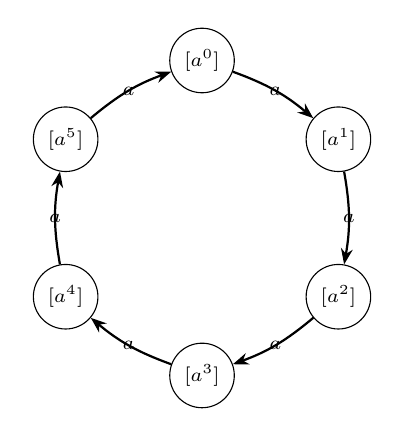
\begin{tikzpicture}[
  node distance=1.2cm,
  every node/.style={draw, circle, inner sep=3pt, minimum size=7mm},
  arr/.style={-{Stealth[length=2mm]}, thick}
]
  \def\n{6}
  \def\radius{2cm}
  \foreach \i in {0,...,5} {
    \node (n\i) at ({90 - 360/\n * \i}:\radius)
      {\scriptsize $[a^{\i}]$};
  }
  \foreach \i [evaluate=\i as \j using {int(mod(\i+1,\n))}] in {0,...,5} {
    \draw[arr] (n\i) to[bend left=10]
      node[draw=none, midway, font=\scriptsize, outer sep=2pt] {$a$}
      (n\j);
  }
\end{tikzpicture}
\caption{The discrete circle $\mathbb{Z}/6\mathbb{Z}$ as a
relational quotient. The law $a^6 \sim \id$ forces closure.}
\label{fig:circle}
\end{figure}

\begin{example}[Distance on the discrete circle]
\label{ex:circle-distance}
Assign $w(a) = 1$. The distance between $[a^j]$ and $[a^k]$ is:
\[
  d\bigl([a^j],[a^k]\bigr)
  = \min\!\bigl(|k-j| \bmod n,\; n - (|k-j| \bmod n)\bigr).
\]
The maximum distance is $\lfloor n/2 \rfloor$, reflecting circular
topology. No coordinates or embedding are used.
\end{example}

\subsection{End-to-End Worked Example: Four-Point Metric Space}
\label{sec:worked}

Let $X = \{p, q, r, s\}$ with
$d(p,q) = d(q,r) = d(r,s) = 1$, $d(p,r) = d(q,s) = 2$,
$d(p,s) = 3$: four equally-spaced collinear points.

Starting from the complete-graph presentation (12 edges), the
edges $e_{pr}, e_{rp}, e_{qs}, e_{sq}, e_{ps}, e_{sp}$ are all
redundant (each has an alternative path of equal weight). The
minimal presentation is the path graph
$\{e_{pq}, e_{qp}, e_{qr}, e_{rq}, e_{rs}, e_{sr}\}$.

The induced metric recovers $d$ exactly:
$d_{\mathrm{ind}}(p,r) = 2$, $d_{\mathrm{ind}}(p,s) = 3$, etc.
The triangle inequality is tight at every triple, which is
precisely the condition for a unique minimal path presentation.

\subsection{The Discrete Torus}
\label{sec:torus}

Let $R = \{a, b\}$ with the congruence generated by:
\[
  a \circ b \sim b \circ a, \quad a^n \sim \id, \quad b^m \sim \id.
\]
By Theorem~\ref{thm:quotient}:
\[
  \RC/{\sim} \cong \mathbb{Z}/n\mathbb{Z} \times \mathbb{Z}/m\mathbb{Z}.
\]

\begin{figure}[h]
\centering
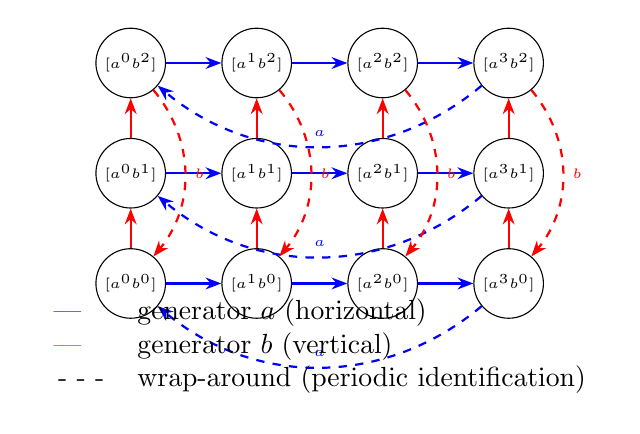
\begin{tikzpicture}[
  arr/.style={-{Stealth[length=2mm]}, thick},
  node/.style={draw, circle, inner sep=2pt, minimum size=5mm,
    font=\scriptsize}
]
  \def\cols{4}
  \def\rows{3}
  \foreach \i in {0,...,3} {
    \foreach \j in {0,...,2} {
      \node[node] (n\i\j) at (\i*1.6, \j*1.4)
        {\tiny $[a^\i b^\j]$};
    }
  }
  \foreach \i [evaluate=\i as \inext using {int(mod(\i+1,4))}]
    in {0,...,3} {
    \foreach \j in {0,...,2} {
      \ifnum\i<3
        \draw[arr, blue] (n\i\j) -- (n\inext\j);
      \else
        \draw[arr, blue, dashed] (n\i\j) to[bend left=40]
          node[draw=none, above, font=\tiny] {$a$} (n0\j);
      \fi
    }
  }
  \foreach \j [evaluate=\j as \jnext using {int(mod(\j+1,3))}]
    in {0,...,2} {
    \foreach \i in {0,...,3} {
      \ifnum\j<2
        \draw[arr, red] (n\i\j) -- (n\i\jnext);
      \else
        \draw[arr, red, dashed] (n\i\j) to[bend left=40]
          node[draw=none, right, font=\tiny] {$b$} (n\i0);
      \fi
    }
  }
  \node[draw=none] at (2.4, -0.8) {
    \begin{tabular}{ll}
      \textcolor{blue}{---} & generator $a$ (horizontal) \\
      \textcolor{red}{---}  & generator $b$ (vertical) \\
      \,{- - -} & wrap-around (periodic identification)
    \end{tabular}
  };
\end{tikzpicture}
\caption{The discrete torus $\mathbb{Z}/4\mathbb{Z} \times
\mathbb{Z}/3\mathbb{Z}$. Dashed arrows indicate periodic
identifications; commutativity $ab \sim ba$ means traversal
order is irrelevant.}
\label{fig:torus}
\end{figure}

\subsection{Relational Curvature via Noncommutativity}
\label{sec:curvature}

Let $R = \{a, b, a^{-1}, b^{-1}\}$ with
$a \circ a^{-1} \sim \id$ and $b \circ b^{-1} \sim \id$.
Define the \emph{relational commutator}:
\[
  [a,b] = a \circ b \circ a^{-1} \circ b^{-1}.
\]
If $[a,b] \sim \id$, the loop closes: the structure is locally
flat. If $[a,b] \not\sim \id$, traversing the loop
$a \circ b \circ a^{-1} \circ b^{-1}$ does not return to the
starting class. This is the discrete relational analogue of
holonomy: the signature of nonzero curvature.

Curvature is a discrete, finitely computable property: check
whether $[a,b] \sim \id$ under the congruence.

\begin{remark}[Relationship to lattice gauge theory]
\label{rem:wilson}
The relational commutator $[a,b] = a \circ b \circ a^{-1}
\circ b^{-1}$ is, in the language of lattice gauge theory, the
Wilson loop around an elementary plaquette~\cite{wilson74}. When
the generators carry values in a Lie group $G$ (the group-valued
extension considered in the companion paper), the commutator
becomes the face holonomy $g^a \cdot g^b \cdot (g^a)^{-1} \cdot
(g^b)^{-1} \in G$, and $[a,b] \sim \id$ is the discrete flatness
condition. The identification of the relational commutator with
holonomy is not new; it is explicit in Wilson~\cite{wilson74}.
What the PRG framework adds is the categorical framing: the
flatness condition $[a,b] \sim \id$ is a congruence relation on
the free category, and quotienting by it is the same operation as
restricting to flat discrete connections.
\end{remark}

\begin{remark}[Algebraic vs.\ metric curvature]
\label{rem:curvature_gap}
Nontrivial commutators detect \emph{failure of local flatness}
at the algebraic level: the loop $a \circ b \circ a^{-1} \circ
b^{-1}$ does not return to its starting class, which is the
discrete analogue of holonomy. However, noncommutativity alone
does not imply negative metric curvature: free groups are highly
noncommutative yet $\delta$-hyperbolic; nilpotent groups are
noncommutative but not hyperbolic. Metric curvature is captured
quantitatively by the triangle defect $\kappa$ of
Proposition~\ref{prop:hyperbolicity}. The commutator
$[a,b] \not\sim \id$ is a necessary algebraic precondition for
curvature; the triangle defect provides the metric measurement.
The two notions coincide --- a nontrivial commutator produces a
nonzero triangle defect --- only under additional geometric
conditions such as local regularity of the presentation.
\end{remark}

\begin{proposition}[Triangle defect and $\delta$-hyperbolicity]
\label{prop:hyperbolicity}
Let $(\mathcal{O}, d)$ be the metric space induced by a relational
system with inverses. Define the \emph{triangle defect}:
\[
  \kappa(x, y, z) := d(x,y) + d(y,z) - d(x,z).
\]
\begin{enumerate}[label=(\roman*)]
  \item If $\kappa(x,y,z) \leq \delta$ for all $x,y,z \in
        \mathcal{O}$, then $(\mathcal{O}, d)$ is
        $O(\delta)$-hyperbolic in the sense of Gromov.
  \item If $(\mathcal{O}, d)$ is $\delta'$-hyperbolic, then
        $\kappa(x,y,z) \leq \delta'$ for all $x,y,z$.
\end{enumerate}
In particular, $\kappa \equiv 0$ characterizes tree-like
($0$-hyperbolic) metric spaces.
\end{proposition}

\begin{proof}
\textit{(i).} Assume $\kappa(x,y,z) \leq \delta$ for all triples,
i.e., $d(x,z) \geq d(x,y) + d(y,z) - \delta$. Take any geodesic
triangle with vertices $x,y,z$ and a point $p$ on side $[x,y]$
with $d(x,p) = a$, $d(p,y) = b$, $a + b = d(x,y)$. Applying the
defect bound to $(x,p,z)$ gives $d(p,z) \leq d(x,z) - a + \delta$.
Comparing with the path $p \to y \to z$ of length $b + d(y,z)$
and using the defect bound for $(x,y,z)$, a standard thin-triangle
argument shows $p$ lies within $2\delta$ of $[x,z] \cup [y,z]$.
Hence triangles are $2\delta$-thin and $(\mathcal{O},d)$ is
$O(\delta)$-hyperbolic. The precise constant relating defect
bounds to the thin-triangle constant depends on the chosen
definition of hyperbolicity; see~\cite{buragoetal} for a careful
account.

\textit{(ii).} If $(\mathcal{O},d)$ is $\delta'$-hyperbolic,
apply the four-point condition with base point $y$:
$d(x,z) + d(y,y) \leq d(x,y) + d(y,z) + \delta'$.
Since $d(y,y) = 0$, this gives $\kappa(x,y,z) \leq \delta'$.
\end{proof}

\subsection{Pseudo-Periodic Examples}
\label{sec:pseudoperiodic}

\begin{definition}[Pseudo-Periodic System]
\label{def:pseudoperiodic}
A relational system with generator $a$ and congruence $\sim$ is
\emph{pseudo-periodic} with period $n$ and shift $\phi$ if
$a^n \sim \phi$ and $\phi \not\sim \id$.
\end{definition}

\begin{example}[Helix]
\label{ex:helix}
Let $R = \{a, b\}$ with $a^n \sim b$ and $b^k \sim \id$.
Each traversal of $n$ steps in $a$ advances one step in $b$;
after $k$ traversals the $b$-direction closes. The quotient
encodes a discrete helix: $n$ steps per turn, $k$ turns before
closure.
\end{example}

\begin{remark}[Connection to semidirect products]
\label{rem:semidirect}
If the shift $\phi$ acts on the cyclic structure by an
automorphism $\varphi$, the resulting quotient is
$\mathbb{Z}/n\mathbb{Z} \rtimes_\varphi \langle \phi \rangle$.
The helix, screw motion, and glide reflection are all semidirect
products of this form.
\end{remark}

\subsection{Negative Curvature: The Infinite Regular Tree}
\label{sec:tree}

Fix $k \geq 2$. Let $V$ be all finite words over $\{1,\dots,k\}$;
for each vertex $v$ and symbol $i$, include $e_{v,i} : v \to vi$
and $\bar{e}_{v,i} : vi \to v$, with unit weights.

\begin{proposition}
The induced metric satisfies
$d(v,w) = |v| + |w| - 2|v \wedge w|$,
where $v \wedge w$ is the longest common prefix.
\end{proposition}

\begin{theorem}[Hyperbolic features]
The $k$-regular tree satisfies: (i) unique geodesics between any
two vertices; (ii) exponential volume growth: $k^n$ vertices at
distance $n$ from the root; (iii) $0$-thin triangles: each side
lies in the union of the other two.
\end{theorem}

\subsection{Positive Curvature: Triangulated Sphere}
\label{sec:sphere}

Let $T$ be a triangulation of $S^2$ with vertex set $V_T$,
edge set $E_T$, and unit weights. The induced metric
$d_T$ counts minimum triangulation edges in any path. The
diameter is finite.

\begin{example}[Geodesic non-uniqueness: icosahedral graph]
\label{ex:icosahedron}
The icosahedral graph has 12 vertices, diameter 3, and
$A_5 \times \mathbb{Z}/2\mathbb{Z}$ symmetry. Any vertex has
exactly 6 shortest configurations of length 3 to its antipodal
vertex: the relational analogue of multiple geodesics between
antipodal points on a positively curved surface.
\end{example}

\subsection{Flat Geometry: Integer Grid}
\label{sec:grid}

Let $V_n = \{0,\dots,n\}^2$ with all 8-connected edges of unit
weight.

\begin{proposition}
The induced metric is the Chebyshev distance:
$d_n((i_1,j_1),(i_2,j_2)) = \max\{|i_1-i_2|, |j_1-j_2|\}$.
\end{proposition}

The two generators $a$ (horizontal) and $b$ (vertical) commute,
$a \circ b \sim b \circ a$, confirming $[a,b] \sim \id$: the
structure is flat. The torus of \Cref{sec:torus} is this grid
with periodic boundary conditions.

% ==================================================================
\section{Categorical Equivalence}
\label{sec:enriched}

\subsection{Lawvere Metric Spaces}

\begin{definition}[Lawvere metric space~\cite{lawvere}]
A \emph{Lawvere metric space} is a set $X$ with
$d : X \times X \to [0,\infty]$ satisfying $d(x,x) = 0$ and
$d(x,z) \leq d(x,y) + d(y,z)$. Symmetry is not required in
general. A classical metric space is a symmetric Lawvere space
with $d(x,y)=0 \Rightarrow x=y$.
\end{definition}

\subsection{Relational Systems as Free Enriched Categories}

\begin{remark}[Generators and relations]
In categorical language, a relational system $(V, R, s, t)$ with
congruence $\sim$ is a \emph{category presented by generators and
relations}: $R$ supplies the generating morphisms and $\sim$
supplies the relations imposed on them. The word \emph{relation}
now carries its categorical meaning --- a law imposed on
composites --- rather than its set-theoretic meaning. This is why
the elements of $R$ are called generators rather than relations
throughout the paper.
\end{remark}

\begin{definition}[Free enriched category]
Given a weighted relational system $(V, R, s, t, w)$, define a
category enriched over $([0,\infty], \geq, +, 0)$ by: objects
are states $V$; hom-value
$\mathcal{C}(x,y) := \min_{\gamma \in \mathrm{Conf}(x,y)} w(\gamma)$
($\infty$ if no path exists). Composition:
$\mathcal{C}(x,z) \leq \mathcal{C}(x,y) + \mathcal{C}(y,z)$.
\end{definition}

\begin{proposition}
$(V, R, s, t, w) \mapsto \mathcal{C}$ defines a well-formed
$([0,\infty], \geq, +, 0)$-enriched category.
\end{proposition}

\begin{theorem}[Universal property]
\label{thm:free_enriched}
The assignment $(V, R, s, t, w) \mapsto \mathcal{C}$ is left
adjoint to the forgetful functor from
$([0,\infty], \geq, +, 0)$-enriched categories to weighted
relational systems.
\end{theorem}

\begin{proof}[Sketch]
Given $(V, R, s, t, w)$ and an enriched category $\mathcal{D}$,
any weight-preserving map $\phi : R \to \mathcal{D}$ extends
uniquely to an enriched functor $\mathcal{C} \to \mathcal{D}$
by sending each configuration to the composite of its images.
\end{proof}

\subsection{Metric Realization Functor}

\begin{definition}[Category of relational systems]
$\mathbf{RelSys}$: objects are weighted relational systems
$(V, R, s, t, w)$; morphisms $F : (V, R, s, t, w) \to
(V', R', s', t', w')$ are maps $F_V : V \to V'$ and
$F_R : R \to R'$ preserving source, target, and satisfying
$w'(F_R(r)) \leq w(r)$ for all $r \in R$.
\end{definition}

\begin{theorem}[Metric realization functor]
\label{thm:metric_functor}
There is a functor $\mathcal{M} : \mathbf{RelSys} \to
\mathbf{LawMet}$ defined by
$\mathcal{M}(V, R, s, t, w) := (V, d)$
where $d(x,y) = \mathcal{C}(x,y)$.
\end{theorem}

\begin{remark}[Two metric levels and their relationship]
\label{rem:twometrics}
The framework carries two distinct metric structures that
must be distinguished.

\textbf{The object metric} (Theorem~\ref{thm:metric}) is defined
on $\RC/{\sim}$: equivalence classes $[C]$ of configurations.
For a single-state system ($|V| = 1$), all configurations are
endomorphisms, $\RC/{\sim}$ is a quotient monoid or group, and
this metric is the word metric of that presentation. The examples
of \Cref{sec:examples} (circle, torus, tree) all operate at
this level.

\textbf{The state metric} (Definition above) is defined on $V$:
the hom-value $\mathcal{C}(x,y)$ measures the minimum-weight
path between states $x$ and $y$. This is the quantity used in
the reconstruction theorem and the categorical equivalence. It
is the Lawvere metric structure on the underlying graph.

\textbf{The bridge:} in the canonical complete-graph presentation
of Theorem~\ref{thm:reconstruction}, where $V = X$ and every
pair of states has a direct generator, the state metric
$\mathcal{C}(x,y)$ recovers the original metric $d(x,y)$
exactly. For multi-state systems the state metric is the
appropriate geometric invariant; the object metric on $\RC/{\sim}$
captures the richer process-equivalence structure within each
hom-class. The categorical equivalence
(Theorem~\ref{thm:equivalence}) operates at the state metric
level; an analogous equivalence at the object metric level
would require tracking hom-sets, which is part of the
framework's open program.
\end{remark}

\begin{theorem}[Equivalence of categories]
\label{thm:equivalence}
Let $\mathbf{RelSys}_\sim$ be $\mathbf{RelSys}$ with metrically
equivalent objects identified. Then:
\[
  \mathbf{RelSys}_\sim \;\simeq\; \mathbf{LawMet}_{\mathrm{fin}}.
\]
\end{theorem}

\begin{proof}
\textbf{Essential surjectivity.} By Theorem~\ref{thm:reconstruction},
every finite metric space arises as $\mathcal{M}(V, R, s, t, w)$.

\textbf{Full faithfulness.} \textit{Injectivity.} If two morphisms
$F_1, F_2$ induce the same map on states, they agree. 
\textit{Surjectivity.} Given 1-Lipschitz
$f : (V, d) \to (V', d')$, work in the canonical complete
presentations: set $F_V = f$ and $F_R(e_{xy}) = e'_{f(x)f(y)}$.
Then $w'(F_R(e_{xy})) = d'(f(x),f(y)) \leq d(x,y) = w(e_{xy})$
by 1-Lipschitz, so $F$ is a morphism inducing $f$.
\end{proof}

% ==================================================================
\section{Compatibility with Classical Geometry}
\label{sec:classical}

\begin{definition}[Metric approximation]
A sequence of relational systems $(G_n, w_n)$ with induced metrics
$(V_n, d_n)$ and maps $\phi_n : V_n \to X$ \emph{approximates}
a compact metric space $(X,d)$ if: (i) $\phi_n(V_n)$ is
$\varepsilon_n$-dense in $X$ with $\varepsilon_n \to 0$; (ii)
$|d_n(x,y) - d(\phi_n(x),\phi_n(y))| \leq \varepsilon_n$.
\end{definition}

\begin{theorem}[Gromov--Hausdorff bridge~\cite{buragoetal}]
\label{thm:ghbridge}
If $(G_n, w_n)$ approximates $(X,d)$, then
$d_{\mathrm{GH}}((V_n, d_n), (X,d)) \to 0$.
\end{theorem}

\begin{proof}
Construct correspondences $\mathcal{R}_n$ from $\phi_n$ and a
near-inverse $\psi_n$. Both maps satisfy
$d(\phi_n(x), z) \leq \varepsilon_n$. The triangle inequality gives
distortion $\leq 3\varepsilon_n$, hence
$d_{\mathrm{GH}} \leq \frac{3}{2}\varepsilon_n \to 0$.
\end{proof}

\begin{corollary}
$S^1$, $S^2$, and $\mathbb{R}^2$ (locally) arise as
Gromov--Hausdorff limits of finite relational systems via
$\mathbb{Z}/n\mathbb{Z}$, geodesic triangulations, and integer
grids respectively.
\end{corollary}

\begin{theorem}[Pointed GH emergence]
\label{thm:pointed_gh}
Let $(G_n, w_n, v_n)$ be a sequence of rooted relational systems
satisfying: (i) uniform local finiteness (degree $\leq D$);
(ii) uniform edge bounds ($a \leq w_n(e) \leq b$);
(iii) rooted local convergence (metric balls stabilize up to
graph isomorphism for each fixed radius). Then $(V_n, d_n, v_n)$
converges in the pointed Gromov--Hausdorff sense to a pointed
metric space $(V, d, v)$.
\end{theorem}

\begin{example}[The $k$-regular tree as pointed GH limit]
\label{ex:tree_pointed_gh}
Let $G_n$ be the finite ball of radius $n$ in $T_k$, with root
$v_0$ and unit weights. The sequence satisfies all three
hypotheses and converges to $(T_k, d, v_0)$.
\end{example}

% ==================================================================
\section{Multi-Object Configurations}
\label{sec:multiobject}

\begin{definition}[Inter-system relations]
Let $(G_A, w_A)$ and $(G_B, w_B)$ be relational systems with
disjoint vertex sets $V_A$, $V_B$. An \emph{inter-system
relational structure} is a weighted directed graph $G_{AB}$
with edges in $V_A \times V_B \cup V_B \times V_A$ and weight
function $w_{AB}$. The \emph{combined relational system} is
$(G_A \sqcup G_{AB} \sqcup G_B, w_A \sqcup w_{AB} \sqcup w_B)$.
\end{definition}

\begin{definition}[Combined metric]
The \emph{combined metric} on $V_A \cup V_B$ is the induced
metric of the combined system:
$d(x,y) = \inf_\gamma w(\gamma)$
over all configurations $\gamma$ in the combined system.
\end{definition}

\begin{theorem}[Space emergence]
\label{thm:space_emergence}
Let $(G_A, w_A)$, $(G_B, w_B)$ be finite relational systems and
$G_{AB}$ an inter-system structure. Then:
\begin{enumerate}[label=(\roman*)]
  \item The combined system induces a finite metric space
        $(V_A \cup V_B, d)$ fully determined by $G_A$, $G_B$,
        and $G_{AB}$.
  \item Different choices of $G_{AB}$ over the same $G_A$, $G_B$
        produce genuinely different combined geometries.
\end{enumerate}
\end{theorem}

\begin{proof}
(i) The combined system is a finite relational system;
Theorem~\ref{thm:metric} applies. (ii) Different $E_{AB}$ and
$w_{AB}$ produce different path sets, hence different infima.
\end{proof}

Special cases: $E_{AB} = \emptyset$ gives metrically disconnected
union; a single bridge gives dumbbell geometry; zero-weight
connections give metric gluing (relational pushout); uniform
bipartite connections give product-like structure; position-varying
weights give discrete warped products.

% ==================================================================
\section{Relationship to Existing Work}
\label{sec:related}

The mathematical structures in this paper belong to a well-developed
tradition. We state explicitly what is reformulated and what is new.

\paragraph{What is reformulated.}
A relational system $(V, R, s, t)$ with congruence $\sim$ is a
category presented by generators and relations in the standard
sense~\cite{maclane, awodey}. The quotient construction
(Theorem~\ref{thm:quotient}) is the universal property of such a
presentation. The metric emergence theorem
(Theorem~\ref{thm:metric}) is, in the single-state case, the word
metric on a group presentation; in the multi-state case it is the
path metric of the Cayley graph of the quotient groupoid. Both
are classical objects in geometric group theory~\cite{graphgeom}.
The categorical equivalence (Theorem~\ref{thm:equivalence}) is a
consequence of Lawvere's identification of metric spaces with
categories enriched over $([0,\infty], \geq, +, 0)$~\cite{lawvere},
combined with the reconstruction theorem. The Gromov--Hausdorff
bridge results (\Cref{sec:classical}) are standard applications
of the GH framework~\cite{buragoetal}.

\paragraph{What is new.}
The formulation of the $(n,k)$ classification in
relational-process language is a restatement of the classical
theory of cyclic monoids~\cite{cliffordpreston} within the
four-layer framework (generators, congruence, quotient, metric).
As a mathematical result, it is an instance of Clifford and
Preston's classification of cyclic semigroups by index and
period~\cite{cliffordpreston}. The \emph{specific contribution}
is making this classical result visible inside a framework that
separates generators from congruences from quotients, which
allows its scope to be stated precisely: the classification
applies to general (non-invertible) single-generator systems;
for invertible systems the result collapses to the elementary
fact that cyclic groups are classified by order
(Corollary~\ref{cor:invertible_classification}). The pointed GH
emergence theorem (Theorem~\ref{thm:pointed_gh}) with its three
explicit conditions is a concrete relational formulation not
present in the metric geometry literature. The domain of
validity theorem (Theorem~\ref{thm:scope}), which organizes the
boundary between exactly representable, GH-approximable, and
out-of-scope spaces, is new as a unified statement.

The identification of the relational commutator with discrete
holonomy (Section~\ref{sec:curvature}) follows Wilson~\cite{wilson74}
and is not new.

\paragraph{The honest summary.}
The machinery is classical. The primary contribution is a
presentation-level semantic framework: geometric structure is
defined at the level of generators and congruence laws, prior to
quotienting, and metric properties arise as invariants of
congruence classes of processes. The framework isolates four
layers --- generators (syntax), congruence (laws), quotient
(objects), metric (emergent distance) --- that are usually
conflated in geometric group theory expositions. The framework
sits within the tradition of geometric group theory, graph
geometry, and enriched category theory as one further development,
not as a replacement for those foundations. The induced metric
coincides with the path metric on the Cayley graph of the
presented groupoid.

\paragraph{An open question the framework makes visible.}
The four-layer separation raises a question that is difficult to
pose in classical treatments, where one typically starts from the
quotient: \emph{what homological structure does a specific
congruence law produce in the nerve of the free category?}

A concrete instance illustrates the point. Consider the free
category on two generators $a, b$ with inverses, and impose the
single commutativity law $b \cdot a \sim a \cdot b$. The nerve
of the free category (before quotienting) has $H_2 = 0$: no
enclosed surface is present. The nerve of the quotient category
has $H_2 \cong \mathbb{Z}$: a torus surface has appeared. The
surface is not a property of the generators $a$ and $b$; it is
a consequence of the single law. Removing the law removes the
surface.

This observation is not new as a fact about the classifying
space of the group $\mathbb{Z}^2$, which is well-known to be the
torus. The relationship between group presentations and the
homology of their classifying spaces is the subject of classical
combinatorial group theory~\cite{lyndonshupp}, developed through
the Fox calculus, identities among relations, and the bar
complex. What the presentation-level framework makes possible is
a \emph{comparison} between the free nerve and the quotient
nerve for each individual law --- a ``before and after'' view
that identifies the homological contribution of each relation
independently. Whether this comparison yields new invariants not
captured by existing methods in combinatorial group theory is
the open question. It appears not to have been studied
systematically in terms of such presentation-level nerve
comparisons, though the individual components (free nerve, bar
complex, group homology) are all classical.

% ==================================================================
\begin{thebibliography}{99}

\bibitem{lawvere}
F.~W.~Lawvere,
``Metric spaces, generalized logic, and closed categories,''
\textit{Rendiconti del Seminario Matematico e Fisico di Milano}
\textbf{43}:135--166, 1973.

\bibitem{buragoetal}
D.~Burago, Y.~Burago, and S.~Ivanov,
\textit{A Course in Metric Geometry},
AMS Graduate Studies in Mathematics \textbf{33}, 2001.
\newblock \doi{10.1090/gsm/033}.

\bibitem{cliffordpreston}
A.~H.~Clifford and G.~B.~Preston,
\textit{The Algebraic Theory of Semigroups}, Vol.~1,
AMS Mathematical Surveys \textbf{7}, American Mathematical
Society, 1961. See \S1.2 for the classification of cyclic
semigroups by index and period.

\bibitem{wilson74}
K.~G.~Wilson,
``Confinement of quarks,''
\textit{Physical Review D} \textbf{10}(8):2445--2459, 1974.
The plaquette holonomy formula appears in \S2.

\bibitem{lyndonshupp}
R.~C.~Lyndon and P.~E.~Schupp,
\textit{Combinatorial Group Theory},
Springer, 1977. The Fox calculus and identities among relations
are treated in Chapter~IV.

\bibitem{clrs}
T.~H.~Cormen, C.~E.~Leiserson, R.~L.~Rivest, and C.~Stein,
\textit{Introduction to Algorithms}, 4th ed., MIT Press, 2022.

\bibitem{knuthbendix}
D.~E.~Knuth and P.~B.~Bendix,
``Simple word problems in universal algebras,''
in \textit{Computational Problems in Abstract Algebra},
Pergamon Press, 1970, pp.~263--297.

\bibitem{maclane}
S.~Mac Lane,
\textit{Categories for the Working Mathematician},
2nd ed., Springer, 1998.

\bibitem{awodey}
S.~Awodey,
\textit{Category Theory}, 2nd ed.,
Oxford University Press, 2010.

\bibitem{graphgeom}
R.~Diestel,
\textit{Graph Theory}, 5th ed., Springer, 2017.

\bibitem{causalset}
L.~Bombelli, J.~Lee, D.~Meyer, and R.~D.~Sorkin,
``Space-time as a causal set,''
\textit{Physical Review Letters} \textbf{59}(5):521--524, 1987.

\end{thebibliography}

\end{document}